% Introduction

\chapter{Introduction} % Main chapter title

\label{Introduction} % For referencing the chapter elsewhere, use \ref{Chapter1} 

%----------------------------------------------------------------------------------------

\section{Motivation}

Valve recently released SteamVR which is to work with HTC Vive in order to promote virtual reality in their games. Videogames are the platform for interactive media. In the last few years, starting with Nintendo’s Wii console, companies have started to heavily invest in developing ways for users to interact more intimately with their media, where they become ``one with the game”. 

This movement started with the introduction of \emph{Star Trek}’s holodeck and \emph{X-Men}’s Danger Room, which use holographic images to create another reality within a room. This project is in some ways the opposite of that; the ``game'' is inserted into real life. The game is “augmented” into the current time and place, hence the term \textbf{augmented reality} (AR). Augmented reality is where portions of a graphical user interface from a program is seen in the eyes of a user right then and there through a \textbf{heads up display} (HUD). It is heavily inspired by many first person shooter videogames such as \emph{Halo} and \emph{Call of Duty}. 

Augmented reality can be used in many applications, from a surgeon seeing detailed vital signs of a patient to a soldier keeping track of his teammates. This project looks at a practical application of tracking locations of objects and displaying them on a HUD.

\section{Overview}

\begin{figure}
	\centering
	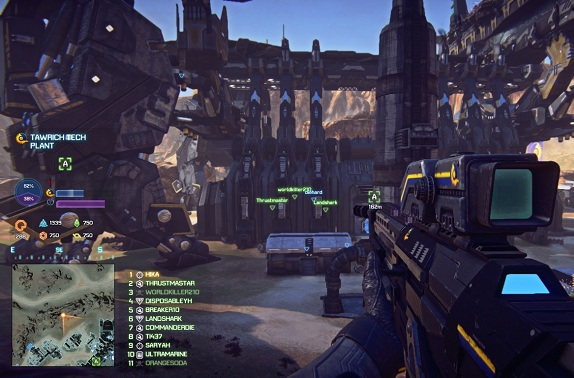
\includegraphics[width=\linewidth]{Figures/GameHUD.jpg}
	\decoRule
	\caption{A screenshot of the videogame \emph{Planetside 2}, showing its HUD. Locations of objectives and allies are indicated with triangles.}
	\label{fig:GameHUD}
\end{figure}

This project takes the visual HUD very popular in video games such as \emph{Planetside 2}, as seen in Figure~\ref{fig:GameHUD}, and reproduces it for use in the actual real world.  While there are many applications and ideas for a heads up display, the project is focused on a proof of concept locating and tracking certain objects within the display. With further development and investment, the project could be expanded and improved upon for many applications. For example, keeping track of a person’s pulse while a surgeon is performing surgery or the marking of a driver's destination on their windshield.

To locate a target, devices called tags are used to mark objects or locations of interest. Each tag is affixed to the target that is to be tracked. The tags determine their distances to other tags, and these distances are triangulated and the positions of tracked objects determined. For 3D positioning, a minimum of four tags are necessary to precisely pinpoint an object's location.

There are three main parts to this project: 
\begin{itemize}
	\item Rangefinding (Chapters~\ref{Rangefinding} and \ref{RangefindingHardware}): rangefinding uses tags to determine the ranges (distances) between other tags.
	\item Position calculation (Chapter \ref{PositionCalculation}):pPosition calculation involves processing the range data from the tags to produce positions in 3D space for use within the augmented reality portion of the project.
	\item Augmented reality rendering (Chapter \ref{AugmentedReality}): the AR subsystem marks the locations of tracked targets on the screen.
\end{itemize}

[Insert image of cellphone screen with arrows and tag locations]

[insert image of tags here]
